\documentclass[12pt,a4paper,oneside,titlepage,listof=totoc,bibliography=totoc]{scrreprt}
\usepackage{scrhack}
\usepackage[top=2.5cm,bottom=2.5cm,left=2.5cm,right=2.5cm,includehead,includefoot,headsep=1cm]{geometry}
\usepackage{iftex}
\ifPDFTeX
    \usepackage[utf8]{inputenc}
    \usepackage[T1]{fontenc}
    \usepackage{lmodern}
    \usepackage[ngerman]{babel}
\fi
\ifLuaTeX
    \usepackage{fontspec}
    \setmainfont{CMU Serif}
    \usepackage{polyglossia}
    \setdefaultlanguage[spelling=new,babelshorthands=true]{german}
\fi
\ifXeTeX
    \usepackage{fontspec}
    \setmainfont{CMU Serif}
    \usepackage{polyglossia}
    \setdefaultlanguage[spelling=new,babelshorthands=true]{german}
\fi
\usepackage{graphicx}
\usepackage{hyperref}
\usepackage{setspace}
\usepackage[headsepline]{scrlayer-scrpage}
\usepackage{acronym}
\usepackage{listings}
\usepackage{float}
\usepackage{enumitem}
\usepackage{color}
\usepackage{microtype}
\usepackage[toc, nogroupskip, nonumberlist, nopostdot]{glossaries}
\usepackage{array}
\usepackage{caption}
\usepackage{cite}

% Für Beispieltext
\usepackage{lipsum}
\usepackage{metalogo}

% Infos
\newcommand{\titel}{TITEL}
\newcommand{\untertitel}{UNTERTITEL}
\newcommand{\arbeit}{}
\newcommand{\pruefung}{Bachelor of Science}
\newcommand{\studiengang}{Informatik}
\newcommand{\studienrichtung}{Angewandte Informatik}
\newcommand{\autor}{Jonas Kümmerlin}
\newcommand{\matrikelnr}{}
\newcommand{\kurs}{TINF15B4}
\newcommand{\firma}{UNTERNEHMEN}
\newcommand{\abgabe}{ABGABETERMIN}
\newcommand{\betreuerdhbw}{BETREUER-DHBW}
\newcommand{\betreuerfirma}{BETREUER-FIRMA}
\newcommand{\jahr}{2017}
\newcommand{\code}[1]{\texttt{#1}}
\newcommand{\source}[1]{\caption*{Quelle: {#1}} }
\newcommand{\zitat}[1]{"`#1"'}

% Logos
\newcommand{\logodhbw}{
\includegraphics[width=6cm]{img/logos/dhbw}}
\newcommand{\logofirma}{
\includegraphics[width=6cm]{img/logos/dhbw}}

% Definition der Kopf- und Fußzeilen
\ihead{\sffamily \autor}
\chead{}
\ohead{\sffamily \headmark}
\automark{section}
\cfoot{\sffamily \pagemark}
\ifoot{}
\ofoot{}

\onehalfspacing

%code style for listings
\definecolor{javared}{rgb}{0.6,0,0} % for strings
\definecolor{javagreen}{rgb}{0.25,0.5,0.35} % comments
\definecolor{javapurple}{rgb}{0.5,0,0.35} % keywords
\definecolor{javadocblue}{rgb}{0.25,0.35,0.75} % javadoc

% Change that for your favorite language
\iffalse
\renewcommand{\lstlistingname}{Programmcode}
\lstset{language=[x86masm]Assembler,
	basicstyle=\ttfamily\footnotesize,
	keywordstyle=\color{javapurple}\bfseries,
	stringstyle=\color{javared},
	commentstyle=\color{javagreen},
	morecomment=[s][\color{javadocblue}]{/**}{*/},
	tabsize=4,
	showspaces=false,
	showstringspaces=false,
	frame=single,
	breaklines=true,
	captionpos=b
}
\fi

\setlist[2]{noitemsep}

\begin{document}
\pagenumbering{roman}

\begin{titlepage}
\sffamily

% Logos
\logodhbw \hfill \\[2ex]

\begin{center}

% Text
\huge{\textbf{\titel}}\\
\Large{\textbf{\untertitel}}\\[4ex]

\LARGE{\textbf{\arbeit}}\\[4ex]

\normalsize{Für die Prüfung zum\\
\pruefung}\\[4ex]

\Large{Studiengang \studiengang}\\
\normalsize{Studienrichtung \studienrichtung}\\
\normalsize{Duale Hochschule Baden-Württemberg Karlsruhe}\\[4ex]

Von\\
\autor \\[8ex]

% Tabelle
\begin{tabular}{ll}
Abgabedatum:				   	& \quad \abgabe\\
%Matrikelnummer: 			    & \quad \matrikelnr\\ 
Kurs:                           & \quad \kurs\\ 
Ausbildungsfirma:	 			& \quad \firma\\
Betreuer der Ausbildungsfirma:  & \quad \betreuerfirma
\end{tabular}
    
\end{center}

\end{titlepage}

\chapter*{Eidesstattliche Erklärung}

Erklärung gemäß~§~5~(3) der "`Studien- und Prüfungsordnung DHBW Technik"' vom 29.~September~2015. Ich versichere hiermit, dass ich diese Arbeit selbstständig verfasst und keine anderen als die angegebenen Quellen als Hilfsmittel verwendet habe.\\[4ex]

\noindent Karlsruhe, den \today \\[8ex]
\noindent \rule{5cm}{0.5pt} \\
\noindent \autor\\

\section*{Sperrvermerk}

Der Inhalt dieser Arbeit darf weder als Ganzes noch in Auszügen Personen außerhalb des Prüfungsprozesses und des Evaluationsverfahrens zugänglich gemacht werden, sofern keine anders lautende Genehmigung der Ausbildungsstätte vorliegt.

\section*{Copyright-Vermerk}

Dieses Werk einschließlich seiner Teile ist \textbf{urheberrechtlich geschützt}. Jede Verwertung außerhalb der engen Grenzen des Urheberrechtsgesetzes ist ohne Zustimmung des Autors unzulässig und strafbar. Das gilt insbesondere für Vervielfältigungen, Übersetzungen, Mikroverfilmungen sowie die Einspeicherung und Verarbeitung in elektronischen Systemen.

\begin{flushright}
    \copyright{} \jahr
\end{flushright}

\clearpage


\tableofcontents
\clearpage


\pagenumbering{arabic}
\setcounter{page}{1}

% Inhalte hier einfügen!
\chapter{Einleitung}

\section{Motivation}

Die Motivation der Arbeit war das Vertiefen der vermittelten, theoretischen Inhalte. Erwartet wurde kein umfangreiches Projekt, sondern nur ein kleines, auf einem 8051 Mikrocomputer lauffähiges Programm, welches ein wenig über den vermittelten Lernstoff hinaus reicht und damit das Wissen um Assembler\cite{bib:assembler} weiter festigt und vertieft.

\section{Aufgabenstellung}

Die Aufgabe war es mit dem erworbenen Wissen aus der Vorlesung \zitat{Systemnahe Programmierung} ein kleines Programm zu entwickeln. Dieses soll dann auf einem 8051 Mikrocomputer mit simulierter Hardware laufen. Die Simulation selbst wird von der verwendeten Entwicklungsumgebung MCU-8051 IDE bereitgestellt. Der 8051 und die IDE werden in Kapitel \ref{section:8051} und \ref{section:ide} genauer vorgestellt.

Wir als Gruppe haben uns das Ziel gesetzt, das bekannte \zitat{Bombenspiel} zu entwickeln. Hierbei wird eine Bombe mit zufälliger Zündschnur zwischen zwei Spielern hin und her geworfen. Der Spieler, bei dem die Bombe explodiert, hat verloren. Das genaue Konzept zu unserer Idee ist in Kapitel \ref{section:konzept} ausführlich erklärt.

\section{Der 8051 Mikrocomputer} \label{section:8051}

Der 8051 Mikrocomputer wurde 1981 von Intel als 8-bit Mikrocontroller auf den Markt gebracht. Es handelt sich um ein \zitat{system on a chip}, was bedeutet, dass RAM, ROM, zwei Timer, ein Serial Port, 4 8-bit Ports und noch einiges mehr auf einem einzigen Chip verbaut sind. Die einzelnen Bestandteile sind in Abbildung \ref{img:8051} dargestellt.\cite{bib:8051}

Mittlerweile ist der Original 8051 veraltet, dennoch existieren viele Abwandlungen (Derivate) beziehungsweise Weiterentwicklungen des 8051. Diese sind allerdings mit höherer Taktfrequenz und geringerer Taktteilung ausgestattet, sodass sie nahezu auf dem aktuellen Stand der Technik und damit deutlich leistungsfähiger als das Ursprungsmodell sind.\cite{bib:8051_2}

\begin{figure}[htbp]
	\centering
	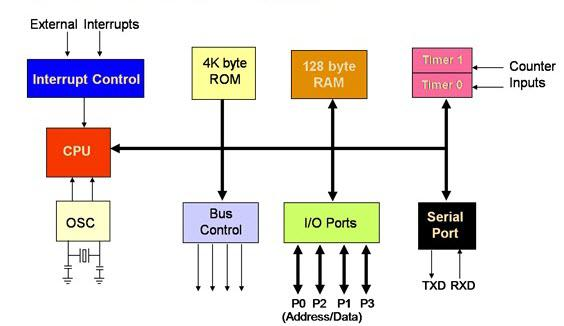
\includegraphics[scale=0.75]{img/8051-diagram}
	\caption{Blockdiagramm eines 8051 Mikrocomputers}
	\label{img:8051}
	\source{https://www.tutorialspoint.com/embedded_systems/images/block_diagram.jpg}
\end{figure}

\chapter{Features}

\section{Kompatibilität}

Die Vorlage funktioniert mit pdf\LaTeX, \XeLaTeX und \LuaLaTeX. Das mitgelieferte \texttt{Makefile}
ruft \XeLaTeX auf.

Die Vorlage ist bereits eingerichtet, um die Verwendung von deutschen Sonderzeichen und
einigen Unicode-Symbolen (z.B. π) zu ermöglichen. Das klappt gut mit \XeTeX und den
\texttt{CMU}-Schriften, sonst eher sporadisch.

Das \texttt{Makefile} wurde nur auf GNU/Linux-Systemen getestet. Es funktioniert wahrscheinlich
auf anderen unixoiden Betriebssystemen, aber eher nicht auf Windows.

\section{Latexrun}

Diese Vorlage benützt \texttt{latexrun}\cite{latexrun}.
Latexrun ruft \LaTeX genau so oft auf wie nötig,
um alle Änderungen der Eingabedateien in die Ausgabedatei zu übernehmen.
Außerdem versucht latexrun, Fehlermeldungen und Warnungen
der richtigen Quelltextdatei und Quelltextzeile zuzuordnen.
Das klappt in den allermeisten Fällen, aber nicht immer. Manchmal kann \texttt{latexrun}
keine Zeilennummer finden, dann muss man den Fehler von Hand suchen.

Das Programm \texttt{latexrun} ist mitgeliefert. Das \texttt{Makefile} ruft \texttt{latexrun}
für alle \texttt{.tex}-Dateien im obersten Verzeichnis auf. Ausgabeformat ist immer PDF.

\section{Dot-Grafiken}

Das Makefile enthält eine Regel zur Konvertierung von Graphen im \texttt{dot}-Format mittels
der GraphViz-Programmsuite \cite{gansner2000open}.

Die Abbildung \ref{fig:dotgraph} zeigt einen sehr einfachen gerichteten Graphen,
der als PDF konvertiert eingebunden ist.

\begin{figure}[!ht]
    \centering
    \caption{Beispielgraph}
    \label{fig:dotgraph}
    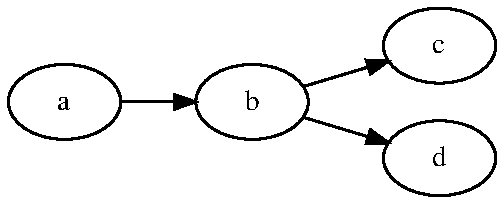
\includegraphics[width=0.8\textwidth]{img/examplegraph}
    \source{Eigene Darstellung}
\end{figure}

\section{SVG-Konvertierung}

Auch integriert ist eine Regel, die SVG-Dateien in von pdf\LaTeX verwendbare PDF-Dokumente konvertiert. Zur Konvertierung wird Inkscape\cite{inkscape} als Kommandozeilenprogramm aufgerufen.
Ein Beispiel-SVG ist in Abbildung \ref{fig:cartman} gezeigt.

\begin{figure}[!ht]
    \centering
    \caption{Beispiel-SVG: Cartman}
    \label{fig:cartman}
    
\includegraphics[width=0.3\textwidth]{img/cartman}
    \source{\url{https://dev.w3.org/SVG/tools/svgweb/samples/svg-files/cartman.svg}}
\end{figure}

\chapter{Blindtext}

\lipsum


\begin{appendix}

\bibliographystyle{apalike}
\raggedright
\bibliography{references/bibliothek}

\noindent
\begin{minipage}{\textwidth}
	\listoffigures
\end{minipage}

\end{appendix}
	
\end{document}
